\chapter{Konzeption}

In diesem Kapitel wird die Konzeption des Gesamtsystems beschrieben. Es wird die Nutzungskontextanalyse beschrieben, welches als Grundlage und Vorbereitung für die anschließende Anforderungsanalyse diente. Die Anforderungsanalyse in welcher, im Rahmen eines Kreativ Workshops, Anwendungsfälle für das zu konzipierende System erarbeitet wurden, wird erläutert. Abschließend wird ein Entwurf der Anwendung beschrieben.

\section{Nutzungskontextanalyse}

% Aktuelle Problemlösungstrategien? Bewertungen auf Online Portalen, Blogs, Interessengruppen, Reklamationen, Technischer Support
Aktuelle Lösungen für die Abgabe von Feedbacks zu Produkten erfolgt oft ohne den Einsatz von Augmented Reality. Diese erfolgen 
oft als Bewertungen in Online Einkaufsportalen, Blog Beiträgen, durch den Austausch in Interessengruppen oder über direkten Kontakt zum Hersteller.

Bei Bewertungen in Onlineportalen, in Blog Beiträgen oder auch bei direktem Kontakt zum Hersteller (z.Bsp. durch E-Mail), haben Kunden die Möglichkeit 
Ihre Feedbacks schriftlich zu beschreiben und mit Bildern oder Videos zu ergänzen. Bei solchen Beschreibungen kommt es jedoch manchmal vor dass 
nicht immer klar hervorgeht zu welcher Stelle oder zu welches Teil am Produkt sich die Beschreibung bezieht. Informationen über die Umgebung in welchem das Produkt 
verwendet wird, geht aus solchen Beschreibungen auch nicht immer hervor. Zudem ist nicht ohne Aufwand möglich direkt zu erkennen an welchen Stellen eines Produktes 
Feedbacks häufen.

Bei Interessengruppen in welchen Nutzer von bestimmten Produkten, sich räumlich zusammentreffen um Erfahrungen auszutauschen wie z.Bsp. zu Hausaltprodukten, Modellflugzeugen, VR Headsets usw., 
haben die Nutzer die Möglichkeit Ihre Ideen genauer zu beschreiben. 
Bei solchen Treffen haben die Nutzer die Möglichkeit mit Bezugnahme auf die Stellen am Produkt und dem Kontext ihrer Umgebung Feedback zum Produkt zu geben. Das Problem bei dieser Art der Rückmeldungen ist jedoch dessen eingrenzte Reichweite. Zudem werden Inhalte welche in solchen Treffen diskutiert wurden oft nicht ausreichend dokumentiert.  

Auf Basis der im Kapitel \ref{CapterFundamentals} behandelten Grundlagen und der Nutzungskontextanalyse wurde eine erste Skizze des Gesamtsystems entworfen in welcher, 
Funktionale wie Nicht-Funktionale Anforderungen an das zu konzipierende System skizziert wird (siehe Abbildung \ref{img:sysstem_sketch}).

\begin{figure}[H]
	\centering
	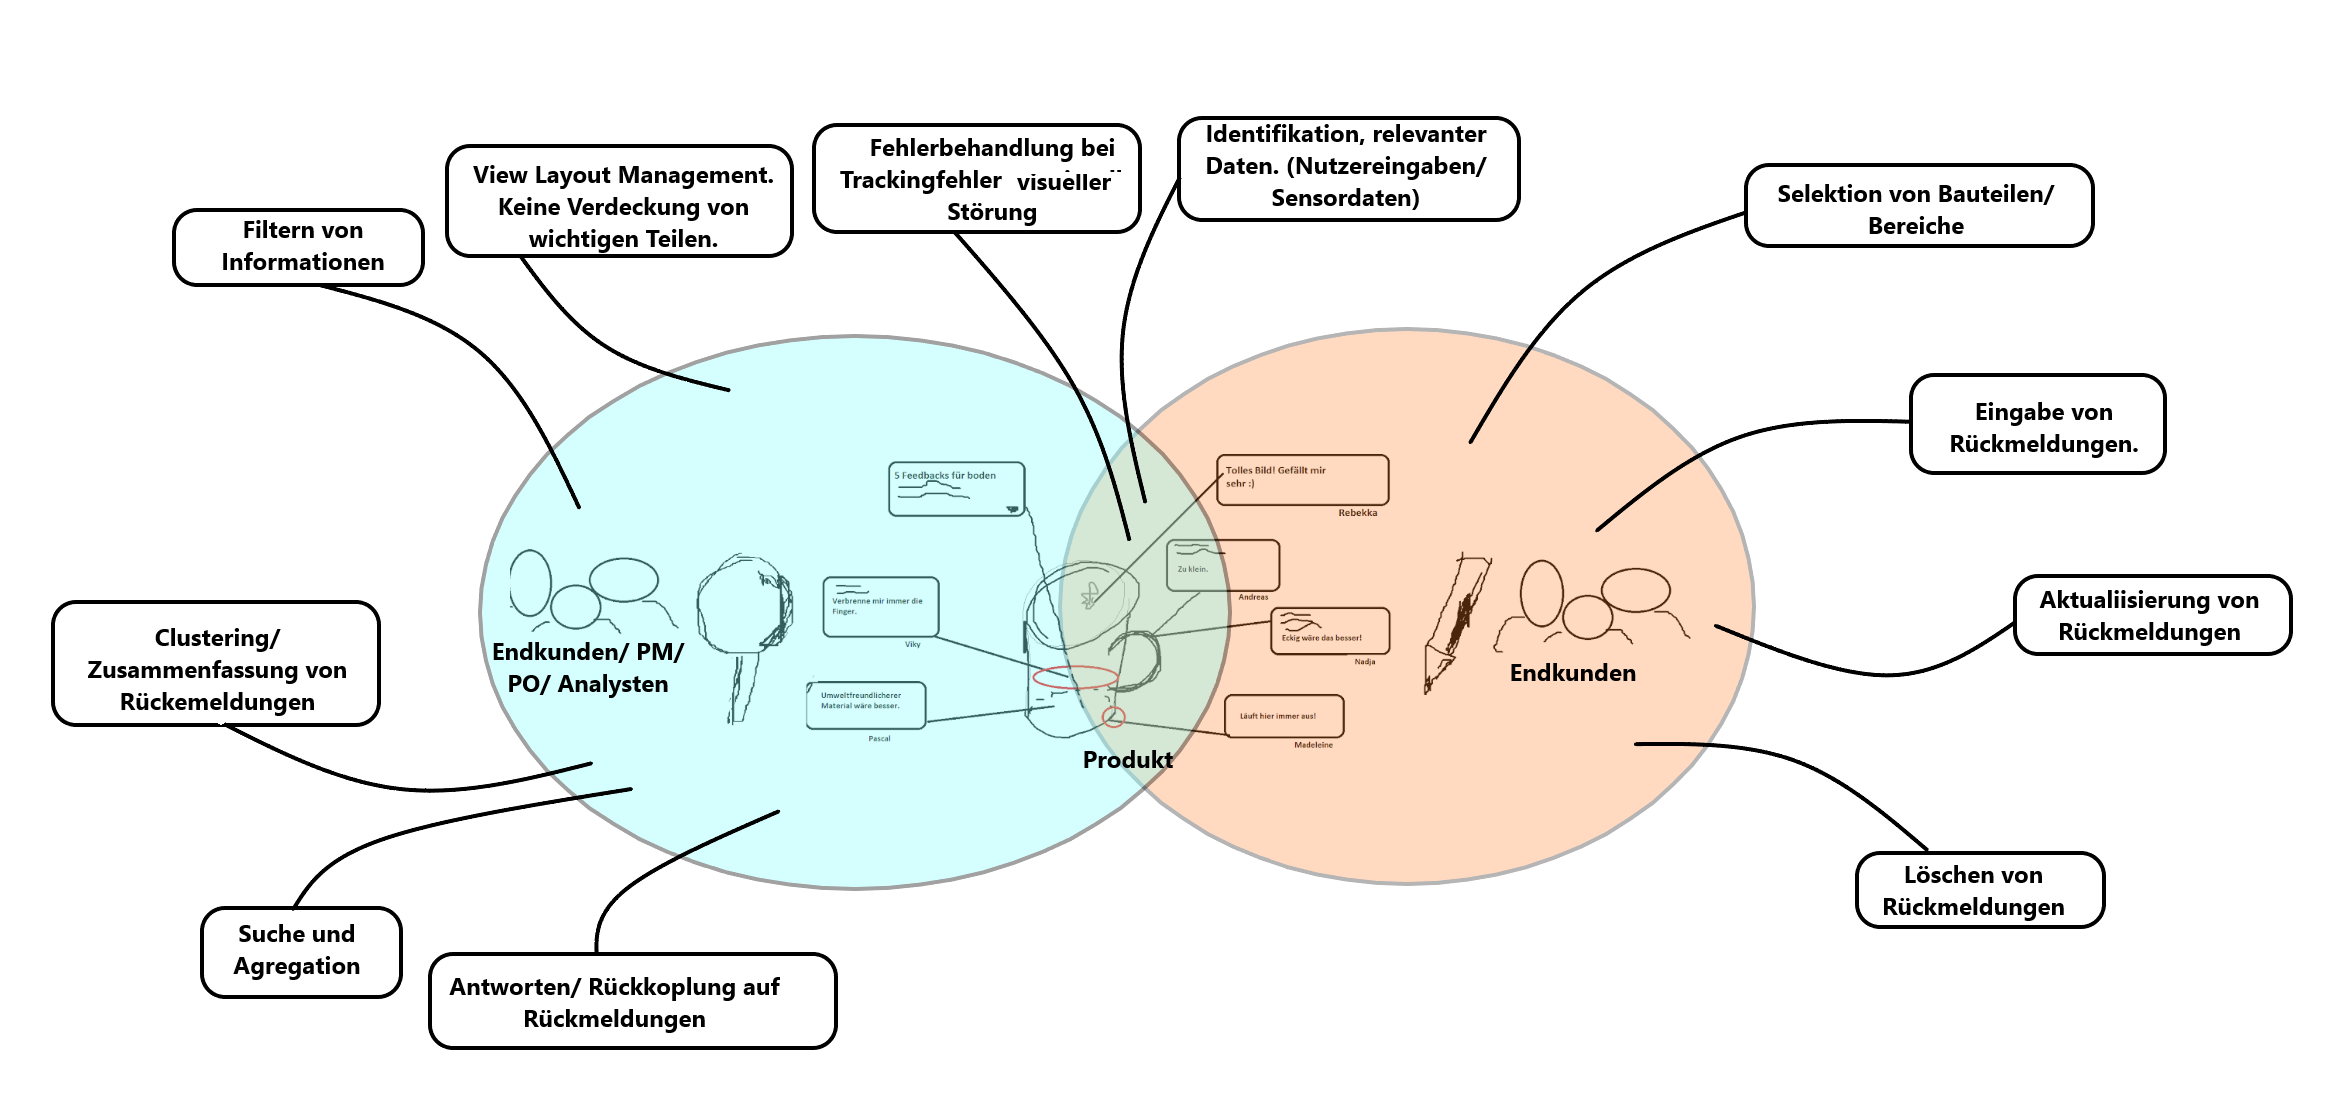
\includegraphics[width=1.0\textwidth]{resources/conception/skizze_gesamtsystem.png}
	\caption{Skizze des Gesamtsystems als erster Entwurf \\Quelle: Eigene Darstellung}
	\label{img:sysstem_sketch}
\end{figure}

Dieses Skizze sollte die Projektidee begreifbarer machen und als grobe Orientierung bei der Anforderungsanalyse dienen.

\section{Anforderungsanalyse}

Die Anforderungsanalyse wurde im Rahmen eines Kreativ Workshops durchgeführt. Ziel des Workshops war es Die Nutzer für das zu konzipierende System zu identifizieren und deren Eigenschaften und Bedürfnisse 
zu analysieren. 

% Vorbereitung
Das Workshop fand am dritten Juli, am Fraunhofer IPK in Berlin statt. Zur Vorbereitung wurde in einem zuvor für diesen Workshop gebuchten, Besprechungsraum, einzelne Stationen \footnote{z.Bsp.: Aufstellung eines Pinnwand für die Erstellung eines Affinitätsdiagrammes, Abbildungen von Personen für die Erstellung von Personas usw.} für die am Workshop durchzuführenden Aktivitäten vorbereitet. 
Zunächst wurden die Teilnehmer begrüßt und für die Teilnahme am Workshop bedankt. Anschließend wurde der Anlass und der Ablauf des Workshop vorgestellt. 

%Durchführung
Mit Hilfe einer kurzen PowerPoint Präsentation wurde die Projektidee vorgestellt und anhand der groben Skizze des zu konzipierenden Systems (Abbildung \ref{img:sysstem_sketch}) verdeutlicht. 
Anschließend fand eine Frage- Antwort Runde statt, welches die Möglichkeit gab, Rückfragen zu stellen und somit sicherzustellen, dass die Projektidee von allen Teilnehmer gleichermaßen verstanden wurde. 

Nach der Vorstellung der Projektidee fand ein Brainstorming statt, dessen Ergebnis in ein Affinitätsdiagramm festgehalten wurden. 
Im gewöhnlichen Vorgang für die Erstellung von Affinitätsdiagramme, schreiben Teilnehmer Ideen auf Kärtchen, welche zunächst unsortiert auf ein Pinnwand geheftet werden. 
Anschließend werden die Ideen, gemeinsam besprochen und in Gruppen bzw. Untergruppen sortiert. In dem stattgefundenen Workshop wurden die Gruppen jedoch im voraus vorgegeben. 

Es sollten Ideen für die Beantwortung folgender Fragen gesammelt werden: 

\begin{itemize}
	\item Wer sind die Nutzer? (Rolle, Erfahrungsstand,  Lebensstil/ Lebenskontext)
	\item Was sind aktuelle Problemlösungsstrategien der Nutzer?
	\item Was sind die Ziele der Nutzer?
	\item Wo liegen die Schmerzpunkte mit aktuellen Lösungstretarien?
\end{itemize}\label{list:AffiDiagramm}

Den Teilnehmern wurde 15 Mintuten Zeit für ein Brainstorming gegeben, indem Ideen zu den, oben genannten Fragen, auf Kärtchen aufschreiben wurden.
Folgende Ideen sind in dabei entstanden (Eine Abbildung des entstandenen Affinitätsdiagramm befindet sich im Anhang [Referenz darauf]): 

\vspace{5mm}
\textbf{Nutzer: } 
Technik Nerd, Produkt Entwickler, Werbeagentur, Unzufriedene, Unerfahrene, Gewerbliche Nutzer/ Laborpersonal, Endkunde, Qualitätsprüfung eines Produkts (Vorgesetzter), Lagerpersonal

\vspace{5mm}
\textbf{Aktuelle Problemlösungsstrategien} 
Email, Chat, Web-Portale, Telefonsupport, Vergleich von Käuferbewertungen

\vspace{5mm}
\textbf{Ziele der Nutzer: } 
Nächstes Produkt sollte besser sein, Eigenes Design, Fehleranfälligkeit beseitigen, Informationen vor dem Kauf, Hilfreiche Bewertungen finden und verstehen, Ersatzteile beschaffen, Lösungen aus dem Nutzerkreis bereitstellen, Infos in Form: Kurzer Beschreibungen/ Kontakt Informationen des Verantwortlichen, Anleitungen, Reklamation Technischer Dokumentationen (Montageanleitung)

\vspace{5mm}
\textbf{Pain-Points: } 
Komplizierte Beschreibung der Umgebung/ Use Case, Zustand der Bearbeitung unbekannt, Fehlerbehebung meines Produktes, Produkt wird nicht wie vorgesehen (geplant) genutzt und funktioniert daher nicht richtig (Vorstellung eines möglichen neuen Anwendungsfalles), Lange Wartezeiten auf Antwort, Bessere Kommunikation zwischen Abteilungen

%Durchführung %Aufbau / Einleitung / Affinitätsdiagram / Personas / Szenarien

%Personas Tabelle

%Name/ Alter / Rolle /Aktuelle Problemlösung / Pain Points

% User Stories


\textbf{User Stories}


%\begin{center}
	\begin{table}[H]
	\caption{User Stories}
	\resizebox{\textwidth}{!}{
	\begin{tabular}{ | c | c | c |c |c |}
		\hline
		\thead{Nr.} & \thead{Als} & \thead{abgeleitet \\ aus \\ Persona} &	\thead{möchte ich} & \thead{damit} \\
		\hline
		10 &  \makecell{Endkunde} & \makecell{Timo} & \makecell{neue Anwendungsfälle \\direkt am Produkt-Teil\\ beschreiben können} &  \makecell{ich bei meiner Beschreibung\\ implizit einen Bezug\\
			zu einer bestimmten\\ Stelle am Produkt\\ herstellen kann} \\
		\hline
		20 &  \makecell{Endkunde} & \makecell{Timo} & \makecell{Ergänzende Anleitungen direkt\\ am Produkt am Produkt Teil\\ oder Stellen ansehen können} &  \makecell{ich mir ergänzende Bemerkungen \\und Anleitungen
			direkt an der \\ betreffenden Stelle ansehen kann
} \\
		\hline
		30 &  \makecell{Endkunde} & \makecell{Timo} & \makecell{Anleitungen zu spezifischen\\ Stellen am Produkt \\beschreiben können} &  \makecell{mir die Bezugnahme zur \\ betreffenden Stelle
			am Produkt\\ erleichtert wird und meine \\Anleitungen
			besser von anderen \\verstanden werden} \\
		\hline
		31 &  \makecell{Endkunde)}  & \makecell{Svenja, \\ Timo, \\ Felix} & \makecell{ein bestimmtes Teil an einem\\
			physischen Produkt auswählen\\
			können
} &  \makecell{ich bezugnehmend auf das ausgewählte\\ Teil
			Aktionen ausführen kann.\\ (z. Bsp.: eine
			Rückmeldung abgeben)}\\
		\hline
		32 &  \makecell{Endkunde}  & \makecell{Svenja, \\ Timo, \\ Felix} & \makecell{eine von mir abgegebene\\
			Rückmeldung auswählen können} &  \makecell{damit ich diese Rückmeldung oder den\\
			Bezugspunkt auf dem physischen Produkt auf das\\
			sich die Rückmeldung bezieht verändern oder\\
			löschen kann}\\
		\hline
		33 &  \makecell{Endkunde}  & \makecell{Svenja, \\ Timo, \\ Felix} & \makecell{die Beschreibung auf einer von mir\\
			abgegebenen Rückmeldung verändern\\
			können.} &  \makecell{ich eine Nachträgliche Korrektur oder Ergänzung\\
			vornehmen zu kann.
}\\
		\hline
		34 &  \makecell{Endkunde}  & \makecell{Svenja, \\ Timo, \\ Felix} & \makecell{den Bezugspunkt (Produkt-Teil oder\\
			bestimmte Stelle auf einem\\
			Produkt-Teil) auf die ein von mir\\
			erstellte Rückmeldung sich bezieht\\
			verändern können.
} &  \makecell{ich eine Nachträgliche Korrektur oder Ergänzung\\
			vornehmen zu kann.
}\\
		\hline
		35 &  \makecell{Endkunde}  & \makecell{Svenja, \\ Timo, \\ Felix} & \makecell{eine von mir erstellte Rückmeldung\\
			löschen können} &  \makecell{ich eine obsolete, redundante oder versehentlich\\
			erstellte Rückmeldung wieder entfernen kann}\\
		\hline
		40 &  \makecell{Endkunde}  & \makecell{Svenja} & \makecell{schnell und unkompliziert\\
			Feedbacks zu Produkt Teile od. Stellen\\
			abgeben können.} &  \makecell{ich auch Feedbacks beiläufig abgeben kann.}\\
		\hline	
		50 &  \makecell{Endkunde}  & \makecell{Svenja, \\ Timo, \\ Felix} & \makecell{möchte ich Bewertungen zu einem\\
			Produkt, am Produkt ansehen können} &  \makecell{ich mich vor dem Kauf eines Produktes genauer\\
			erkundigen kann und mir vor allem für mich\\
			wichtigen stellen am Produkt besser beurteilen\\
			kann
}\\
		\hline	
		60 &  \makecell{Endkunde}  & \makecell{Svenja, \\ Timo, \\ Felix} & \makecell{möchte ich Kontaktinformationen zu\\
			Verantwortlichen Personen sehen\\
			können.} &  \makecell{ich direkt Kontakt zu dieser Person aufnehmen\\
			kann.}\\
		\hline	
		70 &  \makecell{Endkunde}  & \makecell{Timo} & \makecell{möchte ich den Wunsch äußern\\
			können, dass der Hersteller über mein\\
			Feedback informiert wird} &  \makecell{ich sichergehen kann dass mein Feedback\\
			zeitnah vom Hersteller wahrgenommen wird}\\
		\hline	
		80 &  \makecell{Endkunde}  & \makecell{Timo} & \makecell{möchte ich bei Abgabe eines Feedbacks,\\ den
			Einfluss auf mein Geschäft\\
			beschreiben können} &  \makecell{damit ich dem Hersteller des Produktes\\ ein besseres Verständnis über den Ausmaßes ermöglichen\\ kann und dieser den im Feedback beschriebenen\\ Sachverhalt entsprechend beurteilen und priorisieren kann }\\
		\hline	
\end{tabular}}
\end{table}
%\end{center}

%	20 &  \makecell{Geschäftskunde \\ (gewerblich \\ nutzender \\ Endkunde)}  & \makecell{Svenja, \\ Timo, \\ Felix} & \makecell{Text text text  \\ text text text text text} &  \makecell{Text text text  \\ text text text text text} \\
%\hline


\section{Entwurf}

\subsection{Szeanrien}
\subsection{Low-Fidelity-Prototyp}
\subsection{Konzeptioneller Entwurf und Klassendiagramme}

Systemkomponente

Entity Relationship Diagramm (ERM)


Klassendiagramm